\subsection{Detection Rates}
In Figure~\ref{fig:detection_rates}, we show the expected number of LISA detections for each model variation. We find that on average, for our fiducial model, a four year LISA mission will detect 26 BHBH, 27 BHNS and 11 NSNS binaries. Increasing the LISA mission length to ten years changes the number of detections to 42, 45 and 19 respectively.

\begin{figure*}[p]
    \centering
    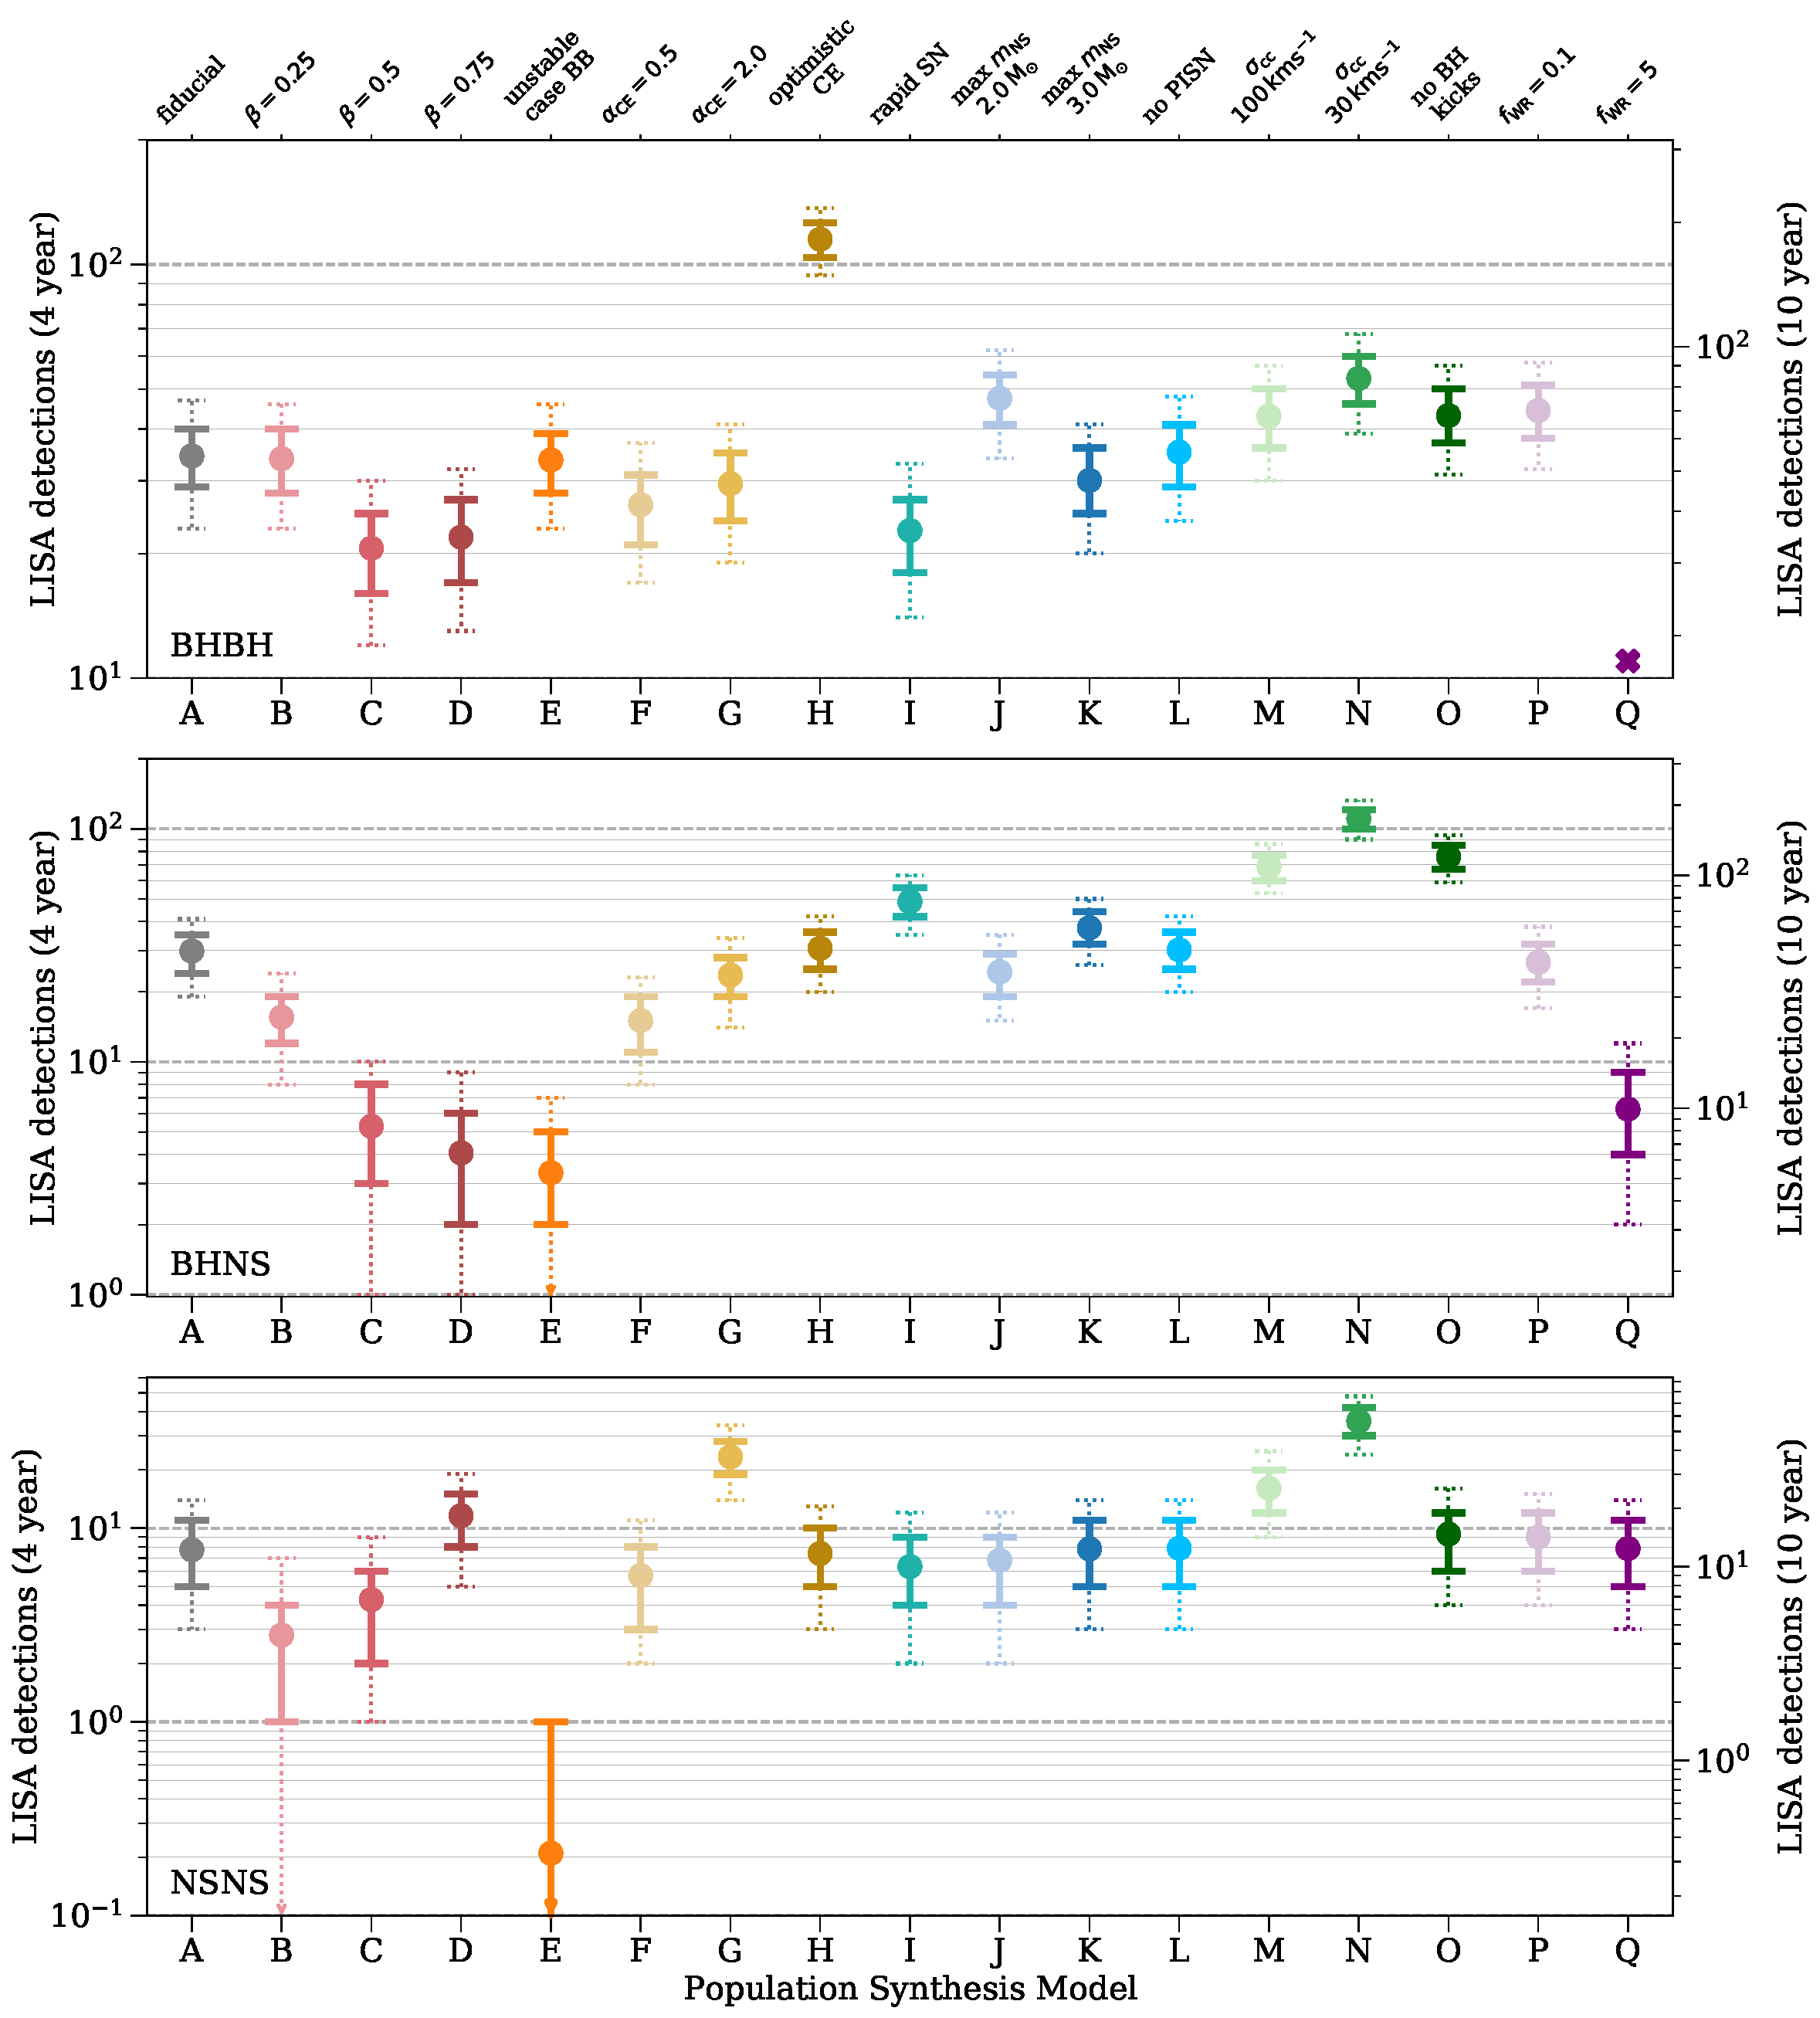
\includegraphics[width=\textwidth]{dco_detections.pdf}
    \caption{The number of expected detections in the LISA mission for different DCO types and model variations. Error bars show the 1 (solid) and 2 (dotted) $\sigma$ uncertainties. The left axis and grid lines show the number of detections in a four year LISA mission and the right axis shows an approximation of the number of detections in a 10 year mission (we scale the axis by $\sqrt{T_{\rm obs}}$, see Table~\ref{tab:detection_rates} for exact rates). Each model is described in further detail in Table~\ref{tab:physics_variations} and details of the fiducial assumptions are in  Section~\ref{sec:fiducial_physics}}
    \label{fig:detection_rates}
\end{figure*}

\subsubsection{BHBH detection rate trends}
The BHBH detection rate is markedly robust across physics variations, with the expected detections in each model staying within 25\% of the fiducial rate (with the exception of model \modOpt{}). Thus even if there are changes in our understanding of the underlying physics before the LISA mission commences, the expected BHBH detection rate is unlikely to change significantly.

The exception to this statement is \modOpt{}, in which we allow Hertzsprung gap donors to survive common envelope events. A large fraction of the progenitors of BHs in this mass range expand significantly during the Hertzsprung gap phase and initiate common envelope events. Therefore, though the detectable fraction does not change significantly, the increased population of BHBHs in the Milky Way leads to this model predicting 2.5 times more detections. \tom{Can also mention slight trends in max NS mass and kicks that are explain in next paragraph}

\subsubsection{BHNS detection rate trends}
In contrast, the BHNS detection rate is very sensitive to changes in binary physics assumptions. Therefore, once LISA flies and we know the actual number of detections, we can compare to each model and possibly provide some constraint on binary evolution physics. There are several notable trends in the BHNS detection rate in the middle pane of Figure~\ref{fig:detection_rates}.

As $\beta$ increases in models \modBetaLow{}-\modBetaHigh{}, the BHNS detection rate steadily decreases. This may seem unintuitive since a higher mass transfer efficiency should lead to more massive compact objects and thus a more detectable population. However, one must also consider that most of these DCOs are formed through a common envelope event and so retaining more of the envelope during mass transfer means that the eventual ejection of the envelope is much more difficult, thus leading to more stellar mergers and fewer detectable BHNSs \citep[e.g.][]{Kruckow+2018}. For a similar reason, the rate is decreased when $\alpha$ is decreased in model \modAlphaLow{}, as this reduces the amount of orbital energy that is used to eject the envelope and thus leads to more stellar mergers. \todo{Why isn't the opposite true for model \modAlphaHigh{}? It seems the number of bound DCOs \textit{does} increase but the merging total decreases...?}

Enforcing that case BB mass transfer is always unstable (model \modCaseBB{}) decreases the detection rate as fewer NSs are produced and thus fewer BHNSs form. This is explained in further detail in Section~\ref{sec:NSNS_detection_trends}. For the same reason as the BHBH rate, model \modOpt{} has a higher number of detections. This change is less prominent than in the BHBH case as the progenitors tend to be lower masses and initiate a CE event less frequently during the Hertzsprung gap phase. 

The Fryer \textit{rapid} prescription (model \modRapid{}) leads to a higher detection rate for BHNSs because progenitors that would become black holes in the \textit{delayed} prescription, instead become neutron stars and so more BHNSs are formed. For the same reason, increasing the maximum neutron star mass increases the detection rate and the inverse is true when it is decreased (in models \modNSLow{} and \modNSHigh{}).

Finally, models \modSigLow{}-\modNoBH{} show increased detection rates as lower kicks result in fewer disrupted binaries and hence a more numerous detectable population. Following this logic it makes sense that model \modSigLower{} produces more detections than model \modSigLow{}. The model with no BH kick (\modNoBH{}) is slightly lower than model \modSigLower{} as the number of surviving binaries is limited by the neutron star kick more than the black hole kick.

\subsubsection{NSNS detection rate trends}\label{sec:NSNS_detection_trends}

\todo{understand the $\beta$ trends}. There is a drastic decrease in detections for model \modCaseBB{} by nearly two orders of magnitude. This is because the majority of NSNS binaries are formed through case BB mass transfer and setting this mass transfer to be always unstable results in many of these binaries to merge before they could become NSNSs. As a result the total number of detections decreases, however interestingly the remaining population represent more massive progenitors (that would not go through case BB mass transfer) and thus is skewed to higher masses and has a \textit{higher} detectable fraction (see Fig.~\ref{fig:detection_fractions}).

\todo{come back to CE ones once we understand the BHNS ones}. \todo{weirdly basically no change in rapid and max NS masses}. As we found in the BHNS trends, a lower value for the core-collapse supernova velocity dispersion increases the detection rate in models \modSigLow{} and \modSigLower{}, whilst changing the BH kick (model \modNoBH{}) of course has no effect on the NSNS population.

\begin{table*}[htb]
    \centering
    \caption{The number of detectable binaries in a 4 and 10 year LISA mission for the 15 different model variations and each DCO type. Each value shows the median and the 90\% confidence interval.}
    \begin{tabular}{c|lll|lll}
        \hline
        \multirow{2}{*}{Model} & \multicolumn{3}{c|}{LISA (4 year)} & \multicolumn{3}{c}{LISA (10 year)} \\ \cline{2-7}
         & \scriptsize{BHBH} & \scriptsize{BHNS} & \scriptsize{NSNS} & \scriptsize{BHBH} & \scriptsize{BHNS} & \scriptsize{NSNS} \\
        \hline
        A & \confinv{25.9}{11.1}{13.6} & \confinv{26.7}{11.9}{14.8} & \confinv{11.3}{6.4}{8.0} & \confinv{42.0}{17.3}{17.3} & \confinv{44.5}{17.8}{20.7} & \confinv{19.3}{8.0}{9.7}\\
        B & \confinv{27.7}{12.6}{12.6} & \confinv{12.0}{6.0}{7.5} & \confinv{4.7}{2.7}{3.3} & \confinv{42.7}{17.6}{17.6} & \confinv{19.5}{7.5}{10.5} & \confinv{8.0}{3.3}{4.0}\\
        C & \confinv{20.6}{9.4}{11.3} & \confinv{6.2}{2.8}{3.4} & \confinv{5.5}{2.7}{4.1} & \confinv{33.8}{13.1}{13.1} & \confinv{10.1}{3.9}{3.9} & \confinv{9.6}{4.1}{4.1}\\
        D & \confinv{20.0}{8.3}{10.0} & \confinv{3.2}{1.6}{1.6} & \confinv{14.6}{8.3}{10.4} & \confinv{31.7}{11.7}{11.7} & \confinv{5.1}{1.9}{2.2} & \confinv{22.9}{10.4}{12.5}\\
        E & \confinv{24.4}{12.2}{14.7} & \confinv{6.8}{3.8}{3.8} & \confinv{0.2}{0.1}{0.1} & \confinv{41.5}{17.1}{17.1} & \confinv{10.6}{3.8}{5.3} & \confinv{0.4}{0.1}{0.2}\\
        F & \confinv{20.0}{10.0}{10.0} & \confinv{11.5}{6.6}{8.2} & \confinv{8.1}{3.6}{5.4} & \confinv{30.0}{12.0}{14.0} & \confinv{19.7}{9.9}{9.9} & \confinv{13.6}{5.4}{6.3}\\
        G & \confinv{25.7}{9.9}{13.8} & \confinv{23.3}{10.6}{10.6} & \confinv{26.5}{15.1}{18.9} & \confinv{39.5}{13.8}{15.8} & \confinv{36.1}{12.7}{17.0} & \confinv{45.4}{18.9}{22.7}\\
        H & \confinv{63.6}{31.8}{47.7} & \confinv{37.4}{20.8}{20.8} & \confinv{14.7}{8.4}{10.5} & \confinv{103.4}{39.8}{55.7} & \confinv{62.3}{24.9}{29.1} & \confinv{25.2}{12.6}{12.6}\\
        I & \confinv{21.7}{10.9}{13.0} & \confinv{56.8}{31.6}{31.6} & \confinv{11.0}{5.5}{6.9} & \confinv{32.6}{13.0}{15.2} & \confinv{94.7}{37.9}{44.2} & \confinv{17.9}{8.3}{8.3}\\
        J & \confinv{32.6}{16.3}{19.6} & \confinv{20.3}{9.0}{13.5} & \confinv{11.0}{6.3}{7.8} & \confinv{52.2}{19.6}{22.8} & \confinv{33.8}{11.3}{15.8} & \confinv{18.8}{7.8}{9.4}\\
        K & \confinv{21.4}{9.7}{11.7} & \confinv{30.6}{13.6}{17.0} & \confinv{11.5}{6.6}{8.2} & \confinv{35.0}{13.6}{15.6} & \confinv{51.1}{20.4}{23.8} & \confinv{19.8}{8.2}{9.9}\\
        L & \confinv{24.7}{9.9}{14.8} & \confinv{26.7}{14.8}{17.8} & \confinv{11.3}{6.4}{8.0} & \confinv{42.0}{14.8}{17.3} & \confinv{44.5}{17.8}{20.7} & \confinv{19.3}{8.0}{9.7}\\
        M & \confinv{29.7}{13.2}{16.5} & \confinv{70.6}{39.2}{39.2} & \confinv{20.4}{11.7}{11.7} & \confinv{46.1}{19.8}{23.1} & \confinv{109.8}{39.2}{54.9} & \confinv{32.1}{14.6}{17.5}\\
        N & \confinv{31.6}{15.8}{19.7} & \confinv{117.7}{58.8}{73.6} & \confinv{51.8}{29.6}{29.6} & \confinv{51.3}{23.7}{23.7} & \confinv{191.3}{73.6}{103.0} & \confinv{81.4}{37.0}{44.4}\\
        O & \confinv{30.2}{15.1}{18.9} & \confinv{96.7}{48.3}{60.4} & \confinv{11.4}{6.5}{8.1} & \confinv{49.1}{22.7}{22.7} & \confinv{157.1}{60.4}{84.6} & \confinv{19.5}{9.7}{9.7}\\
        \hline
    \end{tabular}
    \label{tab:detection_rates}
\end{table*}

\subsection{Distribution on the sensitivity curve}

We illustrate the distribution of detectable DCOs on the sensitivity curve in Figure~\ref{fig:dcos_on_sc}. The shape of the distributions are bounded by the edge of the Milky Way and the scarcity of nearby DCOs. We indicate this with lines of constant distance that form as a boundary for the majority of DCOs, where the remaining scatter is due to variations in mass since lines are plotted for the average chirp mass of each respective DCO. The top edge is not a hard cutoff but is present because for any given distance there is a lower probability of drawing higher frequencies (since binaries spend more time at lower frequencies).

\begin{figure*}[t]
    \centering
    \includegraphics[width=\textwidth]{dcos_on_sc.png}
    \caption{Density distribution of detectable DCOs plotted over the LISA sensitivity curve \citep{Robson+2019}. We plot the total signal of binaries at their dominant frequency $n f_{\rm orb}$, such that $n$ is the harmonic that produces the most relative gravitational wave luminosity ($n = 2$ for circular binaries). If the density of points is below our lowest contour (2\%) then we plot the points as scatter points, where their sizes corresponds to their STROOPWAFEL weights. In order to explain the edges of the distribution, we additionally plot lines of constant distance. The dotted lines show the signal for a circular binary of average chirp mass, whilst the dashed line shows the signal for a binary with $e = 0.9$}
    \label{fig:dcos_on_sc}
\end{figure*}


\subsection{Distributions for the fiducial model}\label{sec:fiducial_distributions}

In Figure~\ref{fig:fiducial_pdf_distributions}, we show the distribution of the individual parameters of the population of detectable binaries and discuss the various features in the following sections.

\subsubsection{Black Hole Mass}
For both the BHBHs and BHNSs, the black hole mass distribution extends across relatively low masses, with $83\%$ and $90\%$ respectively below $10 \unit{M_{\odot}}$. This is because, at the high metallicities in the Milky Way, stellar winds are much stronger and strip away much of the stellar mass before BH formation. The mass distribution also extends down to $2.5 \unit{M_{\odot}}$, our fiducial maximum neutron star mass, since the \citet{Fryer+2012} \textit{delayed} remnant mass prescription does not produce a mass gap between neutron stars and black holes. Thus BHBHs and BHNSs detected by LISA could be ideal for ascertaining whether there exists a lower mass gap between neutron stars and black holes.

The bimodality of the BHBH distribution is a result of most detectable BHBHs in our sample having unequal mass ratios. The two peaks are from the primary and secondary black hole masses and we show their individual distributions with the dotted curves.

The reasoning for these unequal mass ratio is as follows: in order to produce a BHBH, most formation channels require at least the first mass transfer to be stable. This stability is strongly dependent on the mass ratio such that equal mass ratios (at the moment of mass transfer) are preferred for creating BHBHs. Yet, since stellar winds are so strong at high metallicity, and even stronger for more massive stars, the primary star will experience significant mass loss and so an initially \textit{unequal} mass ratio is preferred so that the masses are more balanced at the first instance of mass transfer. Since mass transfer occurs after the end of the main sequence for most of our BHBHs, the star will have a well defined core and these core masses, which go on to form BHs, will reflect the initially unequal mass ratios.

\subsubsection{Neutron Star Mass}
The neutron star mass distribution shows that most neutron stars have low masses, with $69\%$ and $87\%$ having masses below $1.5 \unit{M_{\odot}}$ for BHNSs and NSNSs respectively. The lacks of neutron stars around $1.7 \unit{M_{\odot}}$ and the subsequent small peaks are artifacts of the discontinuous nature of the \citet{Fryer+2012} remnant mass prescription.

\subsubsection{Eccentricity}
The eccentricity distributions show that detectable BHBHs are the most eccentric of the three DCOs. This may seem counter-intuitive since neutron stars receive stronger natal kicks, which cause the orbit to become eccentric. However, these stronger kicks often instead result in disrupted or too-wide binaries. In contrast, BHBHs can receive strong kicks that impart high eccentricity without disrupting and thus tend to be more eccentric. This effect is compounded by the fact that we can see BHBHs at lower orbital frequencies, meaning that they have not had as much time to circularise and so still have significant eccentricity by the time of the LISA mission.

\subsubsection{Orbital Frequency and Frequency Evolution}
The orbital frequency distributions for BHBHs, BHNSs and NSNSs peak at increasing frequencies. This is because a higher mass DCO at the same distance and eccentricity requires a lower frequency to produce the same signal-to-noise ratio and thus be detected. The BHBH distribution also has a tail that extends to $4 \times 10^{-6} \unit{Hz}$, which is comprised of highly eccentric binaries since eccentricity moves the dominant harmonic to higher frequencies. Similar tails are not as prevalent for BHNSs and NSNSs as they do not have as many eccentric binaries.

\subsubsection{Luminosity Distance}
Each DCO's luminosity distance distribution peaks around $8 \unit{kpc}$ since this is the distance to the centre of the Milky Way and thus the most dense location of DCOs. Each DCO also has a shoulder at lower distances since closer binaries are easier to detect. This shoulder is more prominent for the NSNS distribution since their lower relative masses require a smaller distance in order to be detected on average.

\subsubsection{Inspiral Time}
Each DCO has a strong peak at small inspiral times since higher metallicities lead to tighter binaries and thus shorter inspiral times. \todo{explain the bumps}

\begin{figure*}[htbp]
    \centering
    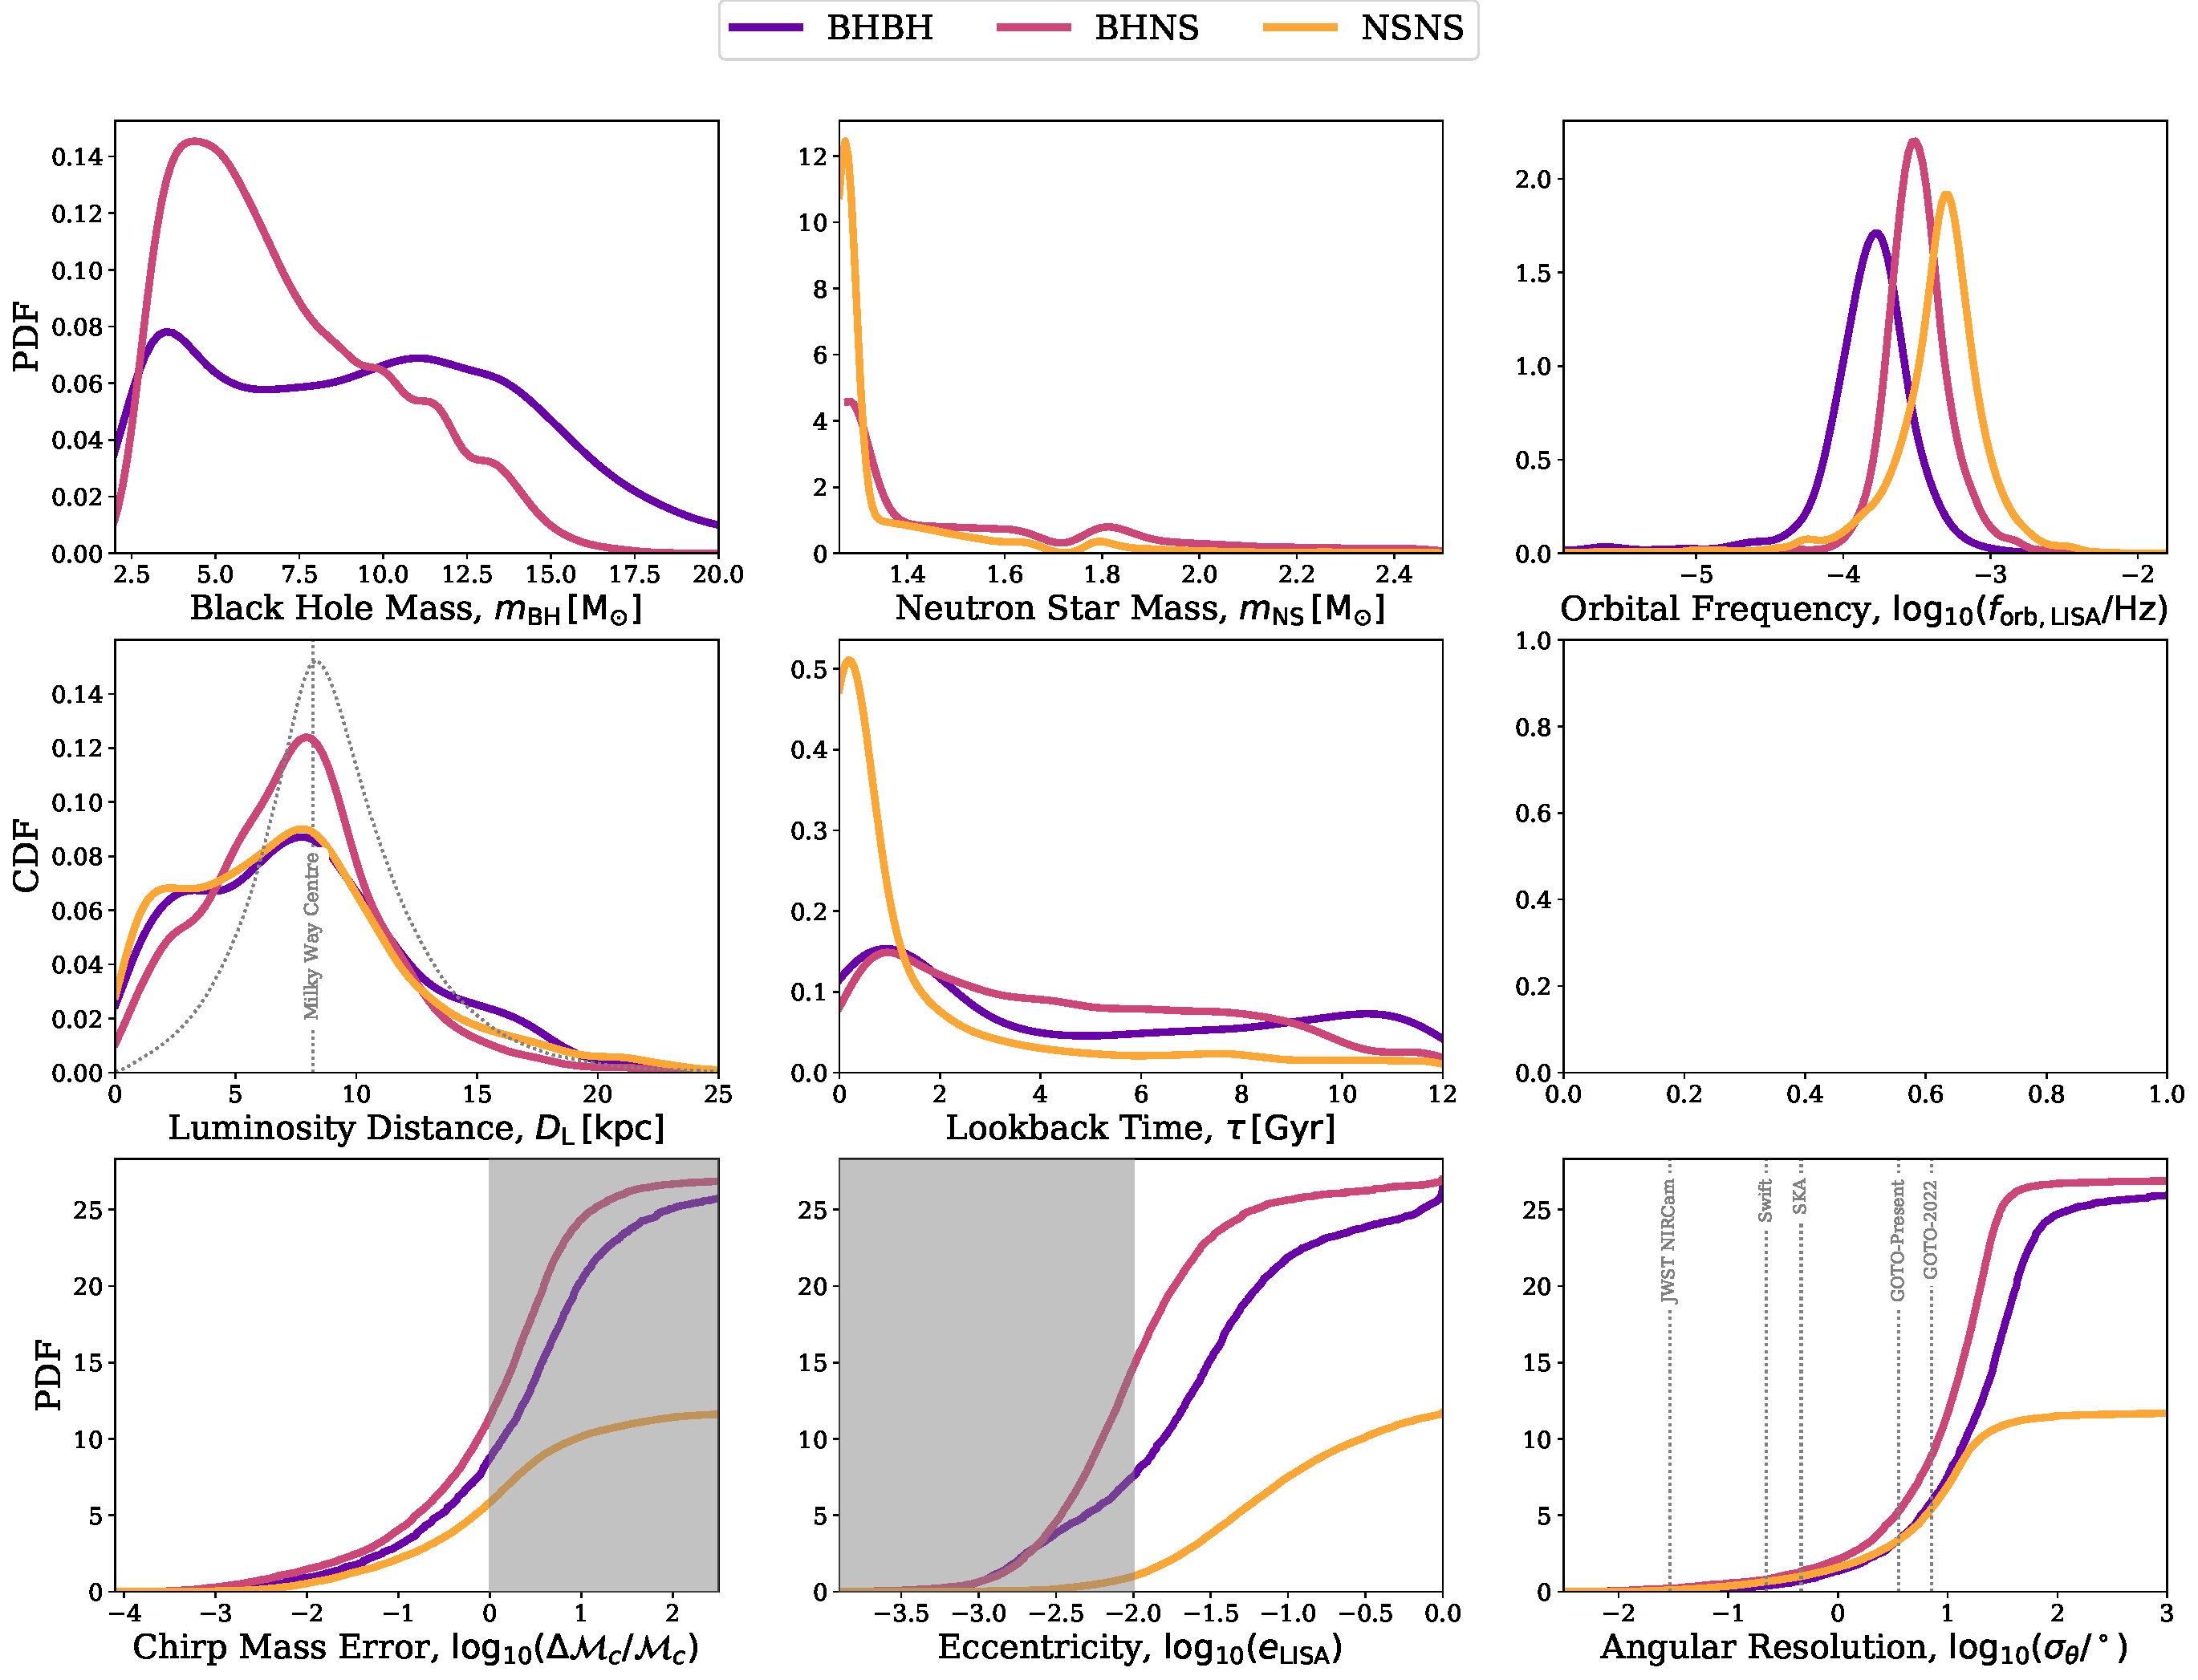
\includegraphics[width=\textwidth]{distribution_grid.pdf}
    \caption{Distributions for various parameters of the binaries that are detectable in a 4 year LISA mission in our fiducial model. Each line represents a kernel density estimator for the distribution and the colour denotes the double compact object type. The dotted curves in the black hole mass distribution show the primary and secondary mass distributions. In Section~\ref{sec:fiducial_distributions} we the features of the distributions.}
    \label{fig:fiducial_pdf_distributions}
\end{figure*}

\subsection{Distinguishing DCOs}
\todo{}

\subsection{Model variations}


\subsection{Comparison with other studies}\label{sec:compare_studies}
\citet{Lau+2020} find that the number of NSNS binaries in the Milky Way that would be detected by a 4 year LISA mission is 33, a factor of three times higher than our fiducial rate. This study incorporates \citet{Lau+2020} uses the same population synthesis code, COMPAS, as this study, though an earlier version. They make several different physical assumptions, using the \citet{Fryer+2012} \textit{rapid} remnant mass prescription, limiting the maximum neutron star mass to $2 \unit{M_{\odot}}$ and not implementing PISN. However, we note that none of these assumptions significantly affect the NSNS LISA detection rate (see bottom panel of Fig.\,\ref{fig:detection_rates}, models \modRapid{}, \modNSLow{} and \modNoPISN{}).

We therefore surmise that the difference between our results is likely due to way in which we simulate the Milky Way. \citet{Lau+2020} assumes constant star formation, solar metallicity and distribute binaries following the blue light luminosity of the Milky Way, whilst we use the distributions from \citet{Frankel+2018} for the star formation rate, metallicity and positions. The \citet{Frankel+2018} star formation rate decreases over time and the metallicity distribution peaks above solar metallicity. Both of these changes could decrease the rate since most NSNS binaries in our sample have short inspiral times compared to the age of the Milky Way and higher metallicity would lead to increased stellar winds and hence less massive DCOs.

\citet{Breivik+2020} find that LISA will detect 93 BHBH, 33 BHNS and 8 NSNS binaries in the Milky Way over a 4 year mission. Although these are significantly different from our fiducial results, we make many different physical assumptions, the most notable being that \citet{Breivik+2020} assumes the optimistic CE scenario. Thus it would be more prudent to compare to our results from model \modOpt{} in which we find 70, 38 and 15 detections respectively. The discrepancy in the NSNS rate is likely due to the fact that we assume that case BB mass transfer onto a NS is always stable but \citet{Breivik+2020} does not and this would significantly decrease our rate (see bottom panel of Fig.\,\ref{fig:detection_rates}, model \modCaseBB{}) . The remaining differences are likely due to using a different population synthesis code (COSMIC) and using a different model for the Milky Way, particularly the assumptions of two fixed metallicities.